\documentclass{article}
\usepackage{float}
\usepackage{amsmath}
\usepackage{amssymb}
\usepackage{graphicx}

\usepackage[top=1in, bottom=1.25in, left=1.25in, right=1.25in]{geometry}

\newcommand{\bs}[1]{\boldsymbol{#1}}
\newcommand{\ul}[1]{\underline{#1}}
\newcommand{\ulbs}[1]{\underline{\boldsymbol{#1}}}
\newcommand{\bsbar}[1]{\boldsymbol{\bar{#1}}}
\newcommand{\ulbsbar}[1]{\underline{\boldsymbol{\bar{#1}}}}
\newcommand{\vbs}[0]{\boldsymbol{v}}
\newcommand{\ebs}[0]{\boldsymbol{e}}

\begin{document}




%%%%%
\section{Perfectly inelastic collision}
\label{sec:prefectly_inelastic_collision}
Two bodies A and B, with known masses and velocities (with A being larger than B) collide and merge with each other. This happens in such a way that A consumes B, resulting in the body A'. The problem is to find the geometry and velocity of the body A'.

\begin{figure}[h]
	\centering
	{\includegraphics{figures/perfectly_inelastic_collision.pdf}}
	\caption{Perfectly inelastic collision.}\label{fig:perfectly_inelastic_collision}
\end{figure}

\subsection{Condition of collision}
The bodies A and B collide if
\begin{equation}
r_A + r_B > d
\end{equation}

\subsection{Geometries after the collision}
Since the bodies fully merge with each other:
\begin{equation}
\begin{split}
A_{A'} &= A_A + A_B\\
r_{A'} &= \sqrt{r_A^2 + r_B^2}
\end{split}
\end{equation}


\subsection{Velocities after the collision}

Conservation of linear momentum:
\begin{equation*}
m_A\vbs_A + m_B\vbs_B = m_{A'}\vbs_{A'}
\end{equation*}
It is assumed that all bodies have the same density $\rho$ and thickness $t$, i.e. $m = \rho t A$, where $A$ is the area. Hence, we have
\begin{equation*}
A_A\vbs_A + A_B\vbs_B = A_{A'}\vbs_{A'}
\end{equation*}
Since the bodies merge with each other, $A_{A'} = A_A + A_B$, thus
\begin{equation*}
A_A\vbs_A + A_B\vbs_B = (A_A + A_B)\vbs_{A'}
\end{equation*}
Solving for $\vbs_{A'}$, we obtain
\begin{equation}
\label{eq:perfectly_inelastic_{A'}ollision}
\vbs_{A'} = \frac{A_A}{A_A + A_B}\vbs_A + \frac{A_B}{A_A + A_B}\vbs_B
\end{equation}




%%%%%
\section{Perfectly elastic collision}
\label{sec:prefectly_elastic_collision}
Two bodies A and B, with known masses and velocities (with A being larger than B) collide and bounce off each other without loss of energy. The problem is to find the velocities of A and B immediately after the collision.

\begin{figure}[h]
	\centering
	{\includegraphics{figures/perfectly_elastic_collision.pdf}}
	\caption{Perfectly elastic collision.}\label{fig:perfectly_elastic_collision}
\end{figure}

\subsection{Velocities after the collision}
In the following, we will make use of a coordinate system aligned with the tangent line of the impacting bodies, consisting of the basis vectors $\ebs_{\perp}$ and $\ebs_{//}$. We can transform to/from this system as follows:
\begin{equation*}
\begin{split}
v_{\perp} &= \vbs\cdot\ebs_{\perp}\\
v_{//} &= \vbs\cdot\ebs_{//}\\
\vbs &= v_{\perp}\ebs_{\perp} + v_{//}\ebs_{//}
\end{split}
\end{equation*}
The basis vector $\ebs_{\perp}$ is normal to the tangent line, but otherwise the direction is arbitrary. The orientation of $\ebs_{//}$ should be such that the resulting system is right-oriented.

In the direction normal to the tangent line of impact, linear momentum is conserved:
\begin{equation}
\label{eq:elastic_collision_momentum_conservation}
m_Av_{A\perp} + m_Bv_{B\perp} = m_Av_{A\perp}' + m_Bv_{B\perp}'
\end{equation}
The velocity component in the direction parallel to the tangent line of impact is unchanged:
\begin{equation}
\begin{split}
v_{A//} &= v_{A//}'\\
v_{B//} &= v_{B//}'\\
\end{split}
\end{equation}
Conservation of kinetic energy:
\begin{equation}
\label{eq:elastic_collision_energy_conservation}
\frac{1}{2}m_A(v_{A\perp}^2+v_{A//}^2) + \frac{1}{2}m_B(v_{B\perp}^2+v_{B//}^2) = \frac{1}{2}m_A(v_{A\perp}'^2+v_{A//}'^2) + \frac{1}{2}m_B(v_{B\perp}'^2+v_{B//}'^2)
\end{equation}
Solving Equations \ref{eq:elastic_collision_momentum_conservation} -- \ref{eq:elastic_collision_energy_conservation} for the velocity components after the collision gives:
%Wolfram Alpha: solve {m*a+n*b==m*A+n*B, c==C, d==D, m*(a^2+c^2)+n*(b^2+d^2)==m*(A^2+C^2)+n*(B^2+D^2)} for {A, B, C, D}
\begin{equation}
\begin{split}
v_{A\perp}' &= \frac{(m_A - m_B)v_{A\perp} + 2m_Bv_{B\perp}}{m_A+m_B}\\
v_{B\perp}' &= -\frac{(m_A - m_B)v_{B\perp} - 2m_Bv_{A\perp}}{m_A+m_B}\\
v_{A//}' &= v_{A//}\\
v_{B//}' &= v_{B//}\\
\end{split}
\end{equation}

If the masses are equal:
\begin{equation}
\begin{split}
v_{A\perp}' &= v_{B\perp}\\
v_{B\perp}' &= v_{A\perp}\\
v_{A//}' &= v_{A//}\\
v_{B//}' &= v_{B//}\\
\end{split}
\end{equation}







%%%%%
\section{Ejection}
A body A with known velocity ejects a body B at a known velocity. We refer to the resulting form of body A (now with diminished mass), as A'. The problem is to find the velocity of the body A'.

\begin{figure}[h]
	\centering
	{\includegraphics{figures/ejection.pdf}}
	\caption{Ejection of mass.}\label{fig:ejection}
\end{figure}

\subsection{Velocities after the ejection}

Conservation of linear momentum:
\begin{equation*}
\begin{split}
m_A\vbs_A &= m_B\vbs_B + m_{A'}\vbs_{A'}
\Rightarrow
\\A_A\vbs_A &= A_B\vbs_B + A_{A'}\vbs_{A'}
\end{split}
\end{equation*}
Since $A_A = A_{A'} + A_B$, we get
\begin{equation*}
A_A\vbs_A = A_B\vbs_B + (A_A - A_B)\vbs_{A'}
\end{equation*}
Solving for $\vbs_{A'}$, we obtain
\begin{equation}
\vbs_{A'} = \frac{A_A}{(A_A - A_B)}\vbs_A - \frac{A_B}{(A_A - A_B)}\vbs_B
\end{equation}







%%%%%
\section{Partial merge}
Two bodies A and B, with known masses and velocities, A being the largest, collide and partially merge with each other such that the larger body A absorbs part of the smaller body B. The result is an enlarged form of body A: A', and a diminished form of body B: B'.

We will denote by C the part of B that is absorbed into A. The area of C is such that after the collision, the bodies are tangentially touching each other. The area of C obviously must be smaller than the area of B.

We denote by $d$ the distance between (the center points of) A and B. Since the positions don't change during the collision process, $d$ is also the distance between A' and B'.

\begin{figure}[h]
	\centering
	{\includegraphics{figures/partial_merge.pdf}}
	\caption{Partial merge of two bodies.}\label{fig:partial_merge}
\end{figure}

\subsection{Condition of collision}
The bodies A and B collide if
\begin{equation}
\label{eq:collision_condition_partial_merge}
r_A + r_B > d
\end{equation}

\subsection{Geometries after the collision}
By nature of the merge process, as described above, we have the following equations:
\begin{equation}
\label{eq:partial_merge_geometrical_relations}
\begin{split}
A_{A'} &= A_A + A_C\\
A_{B'} &= A_B - A_C\\
r_{A'} + r_{B'} &= d
\end{split}
\end{equation}
%
and the following auxiliary conditions:
%
\begin{equation}
\label{eq:partial_merge_auxiliary_conditions}
\begin{split}
A_{A'} &> A_A > A_B > A_{B'}\\
A_C &< A_B
\end{split}
\end{equation}
Substituting $A = \pi r^2$ into Equation \ref{eq:partial_merge_geometrical_relations} and solving for $r_A'$, $r_B'$ and $A_C$ gives:
\begin{equation}
\label{eq:geometries_after_merge_with_plusminus}
\begin{split}
r_{A'} &= \frac{1}{2}\left(d \pm \sqrt{2r_A^2 + 2r_B^2 - d^2}\right)\\
r_{B'} &= \frac{1}{2}\left(d \mp \sqrt{2r_A^2 + 2r_B^2 - d^2}\right)\\
A_C &= \frac{\pi}{2}\left(-r_A^2 + r_B^2 \pm d\sqrt{2r_A^2 + 2r_B^2 - d^2}\right)\\
\end{split}
\end{equation}

A bound on the region of validity of the above equation is given by the condition \ref{eq:partial_merge_auxiliary_conditions}b. In order to express this condition in terms of what is known originally, we insert it into Equation \ref{eq:partial_merge_geometrical_relations}, which gives:
\begin{equation}
\label{eq:region_of_validity}
\begin{split}
A_{A'} &< A_A + A_B\\
A_{B'} &> 0\\
\sqrt{r_A^2 + r_B^2} &< d
\end{split}
\end{equation}
The third equation represents a bound on the region of validity of Equation \ref{eq:geometries_after_merge_with_plusminus}. The other bound is given by Equation \ref{eq:collision_condition_partial_merge}.

We use Equation \ref{eq:partial_merge_auxiliary_conditions}a to resolve ambiguous solutions of the quadratic equations in Equation \ref{eq:geometries_after_merge_with_plusminus}. We also append the aforementioned bounds on the region of validity of the above equations, which finally gives:
\begin{equation}
\label{eq:geometries_after_merge}
\begin{split}
r_{A'} &= \frac{1}{2}\left(d + \sqrt{2r_A^2 + 2r_B^2 - d^2}\right)\\
r_{B'} &= \frac{1}{2}\left(d - \sqrt{2r_A^2 + 2r_B^2 - d^2}\right)\\
A_C &= \frac{\pi}{2}\left(-r_A^2 + r_B^2 + d\sqrt{2r_A^2 + 2r_B^2 - d^2}\right)\\
&\sqrt{r_A^2 + r_B^2} < d < r_A + r_B
\end{split}
\end{equation}

By inserting the two limits of $d$ shown in Equation \ref{eq:geometries_after_merge}d into Equation \ref{eq:geometries_after_merge}c, we can verify that in the limit case of full absorption, $A_C(d = \sqrt{r_A^2 + r_B^2}) = A_B$ and in the limit case of no collision, $A_C(d = r_A + r_B) = 0$.

\subsection{The case of full absorption}
As per Equation \ref{eq:geometries_after_merge}d, full absorption of B into A is given by
\begin{equation}
d <= \sqrt{r_A^2 + r_B^2}
\end{equation}
In this case, refer to Section \ref{sec:prefectly_inelastic_collision}.

\subsection{The case of equality in size between A and B}
TODO



\subsection{Velocities after the collision}
We want to find the velocities of the bodies A' and B'.

We assume that C is released from body B without any impulse or energy transfer between B and C. Thus, the velocity of B is completely unaffected during the collision:
\begin{equation}
\vbs_{B'} = \vbs_B
\end{equation}
Furthermore, the body C will travel with the velocity $\vbs_B$ and be absorbed by A in a perfectly inelastic collision. Thus, from Equation \ref{eq:perfectly_inelastic_collision} we obtain
\begin{equation}
\vbs_{A'} = \frac{A_A}{A_A + A_C}\vbs_A + \frac{A_C}{A_A + A_C}\vbs_B
\end{equation}


\section{Perfectly elastic collision}

\end{document}
